\documentclass{article}
\usepackage{tikz}
\usetikzlibrary{arrows.meta, positioning, quotes}

\begin{document}

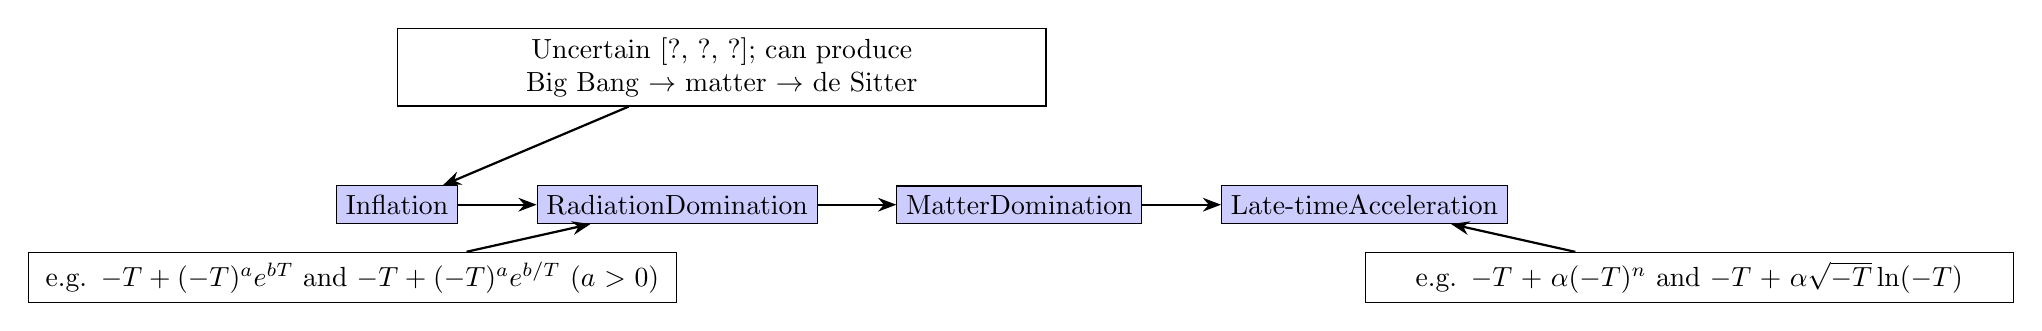
\begin{tikzpicture}[node distance=1cm]
    \node[draw, fill=blue!20] (inflation) {Inflation};
    \node[draw, fill=blue!20, right=of inflation] (radiation) {Radiation\\ Domination};
    \node[draw, fill=blue!20, right=of radiation] (matter) {Matter\\ Domination};
    \node[draw, fill=blue!20, right=of matter] (acceleration) {Late-time\\ Acceleration};

    \node[draw, above=of inflation, anchor=south west, text width=8cm, align=center] (uncertain) {Uncertain [?, ?, ?]; can produce Big Bang $\rightarrow$ matter $\rightarrow$ de Sitter};
    \node[draw, below=of radiation, anchor=south east, text width=8cm, align=center] (examples) {e.g. $-T + (-T)^a e^{bT}$ and $-T + (-T)^a e^{b/T}$ ($a > 0$)};
    \node[draw, below=of acceleration, anchor=south west, text width=8cm, align=center] (examples2) {e.g. $-T + \alpha(-T)^n$ and $-T + \alpha\sqrt{-T}\ln(-T)$};

    \path[->, thick, >=Stealth]
        (inflation) edge [""] (radiation)
        (radiation) edge [""] (matter)
        (matter) edge [""] (acceleration)
        (uncertain) edge [""] (inflation)
        (examples) edge [""] (radiation)
        (examples2) edge [""] (acceleration);
\end{tikzpicture}

\end{document}